% ============================================================
% Draft figure insertions for the final v2 manuscript
% Review placement before copying into main.tex.
% ============================================================

% FIGURE 1
\begin{figure*}[t]
\centering
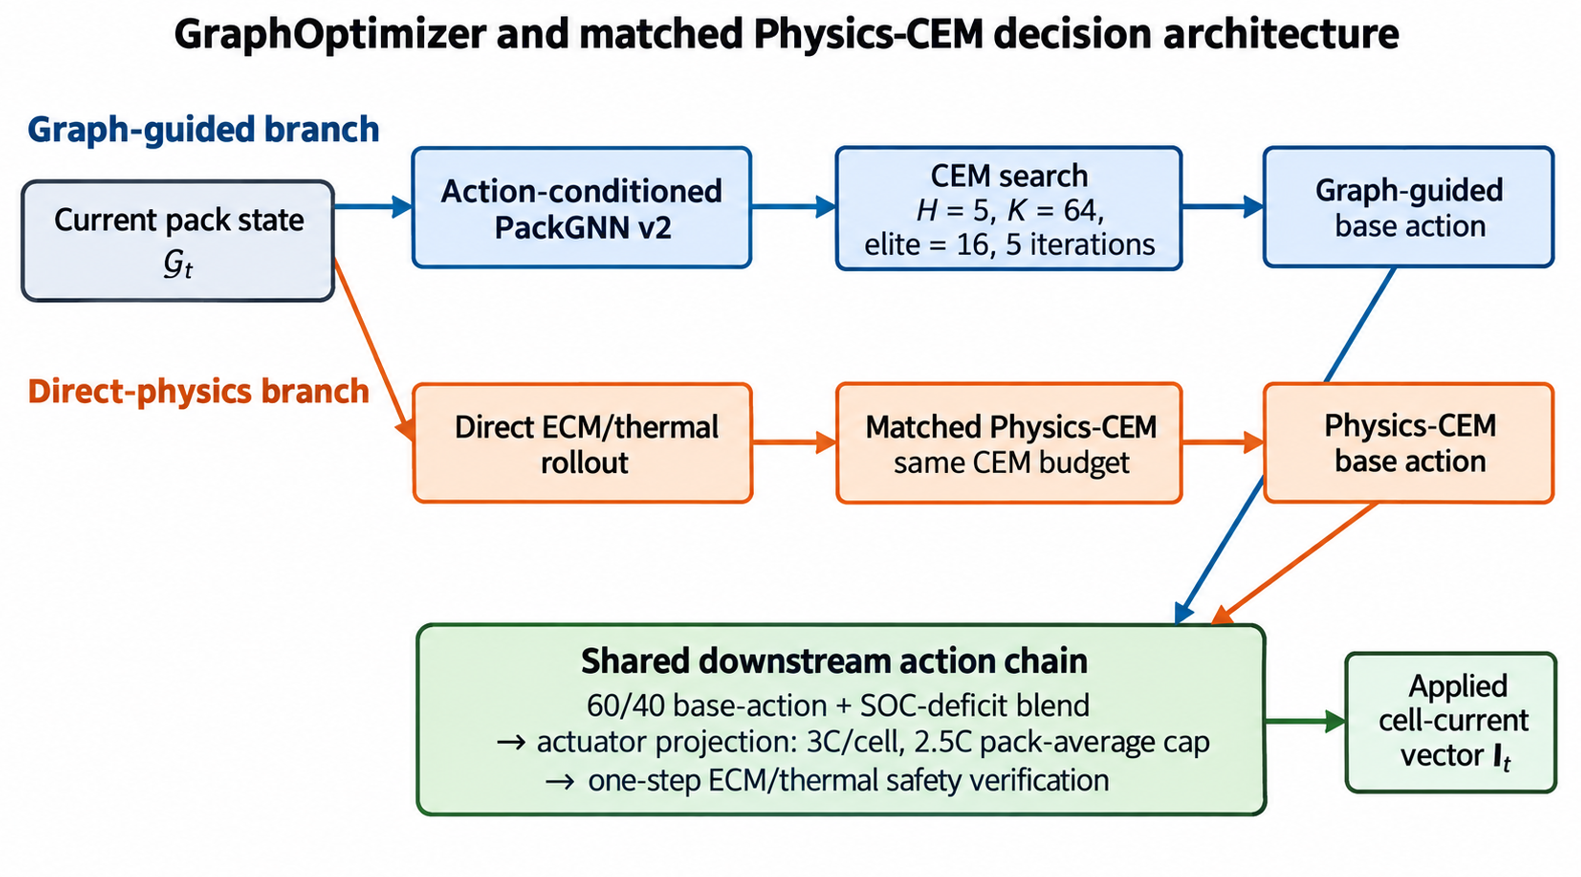
\includegraphics[width=0.94\textwidth]{figures/submission_v2/fig1_controller_architecture.png}
\caption{Final decision architecture for GraphOptimizer and the matched Physics-CEM comparator. Both controllers use the same CEM horizon and sampling budget, 60/40 base-action to SOC-deficit blend, actuator projection, and final one-step model-based safety verification. GraphOptimizer uses action-conditioned PackGNN v2 for candidate ranking and SOC prediction, whereas Physics-CEM uses direct ECM/thermal rollout.}
\label{fig:controller_architecture}
\end{figure*}

% FIGURE 2
\begin{figure}[t]
\centering
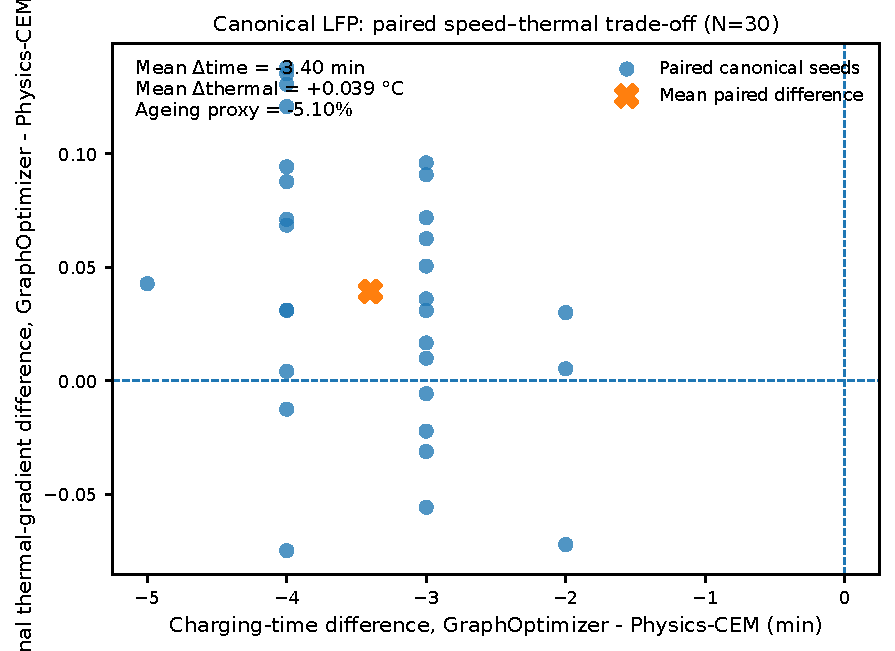
\includegraphics[width=\columnwidth]{figures/submission_v2/fig2_canonical_paired_tradeoff.pdf}
\caption{Paired canonical LFP trade-off for GraphOptimizer relative to matched Physics-CEM across 30 identical initial-pack seeds. Negative horizontal values indicate faster GraphOptimizer charging, whereas positive vertical values indicate a larger final inter-cell thermal gradient. The cross marks the mean paired difference.}
\label{fig:canonical_tradeoff}
\end{figure}

% FIGURE 3
\begin{figure}[t]
\centering
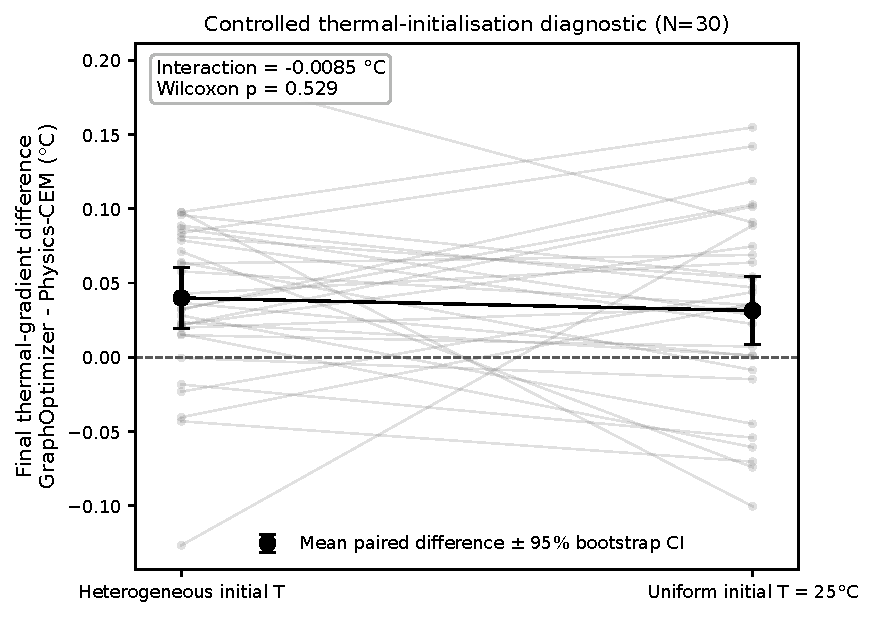
\includegraphics[width=\columnwidth]{figures/submission_v2/fig3_thermal_initial_condition.pdf}
\caption{Controlled thermal-initialisation diagnostic. Each line connects the GraphOptimizer-minus-Physics-CEM final thermal-gradient difference for the same diagnostic pack seed under heterogeneous and uniform 25~$^\circ$C initial cell temperatures. Crosses show paired means with 95\% bootstrap confidence intervals. The thermal-gradient disadvantage persists under uniform initialisation, while the interaction is not statistically significant.}
\label{fig:thermal_initial_condition}
\end{figure}

% FIGURE 4
\begin{figure}[t]
\centering
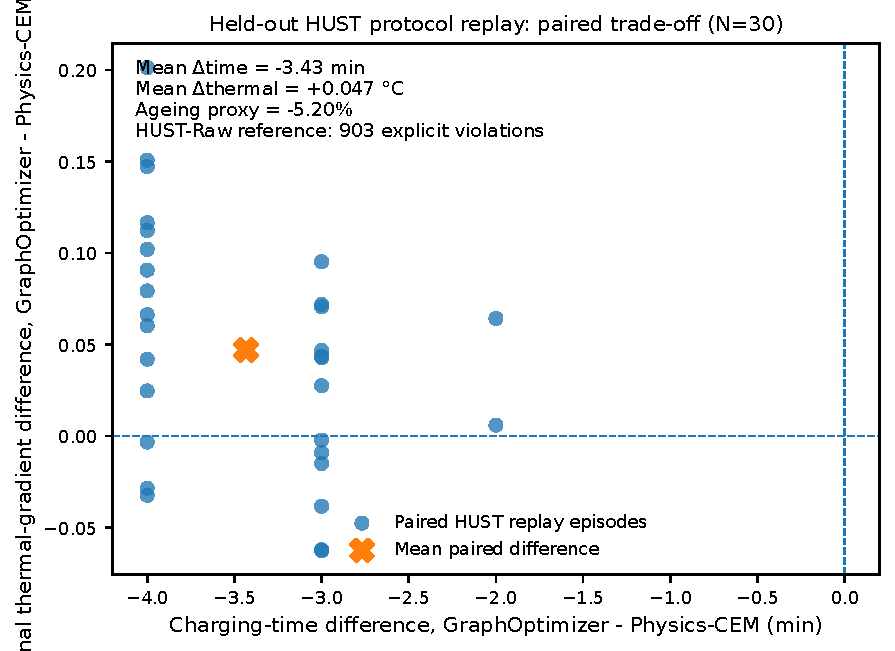
\includegraphics[width=\columnwidth]{figures/submission_v2/fig4_hust_paired_tradeoff.pdf}
\caption{Paired GraphOptimizer-minus-Physics-CEM trade-off in the held-out HUST measured-current protocol replay. The directional pattern reproduces the canonical result: shorter charging time for GraphOptimizer is accompanied by a larger final inter-cell thermal gradient. HUST-Raw is an external-protocol reference and is not an actuator-matched controller comparator.}
\label{fig:hust_tradeoff}
\end{figure}

% FIGURE 5
\begin{figure}[t]
\centering
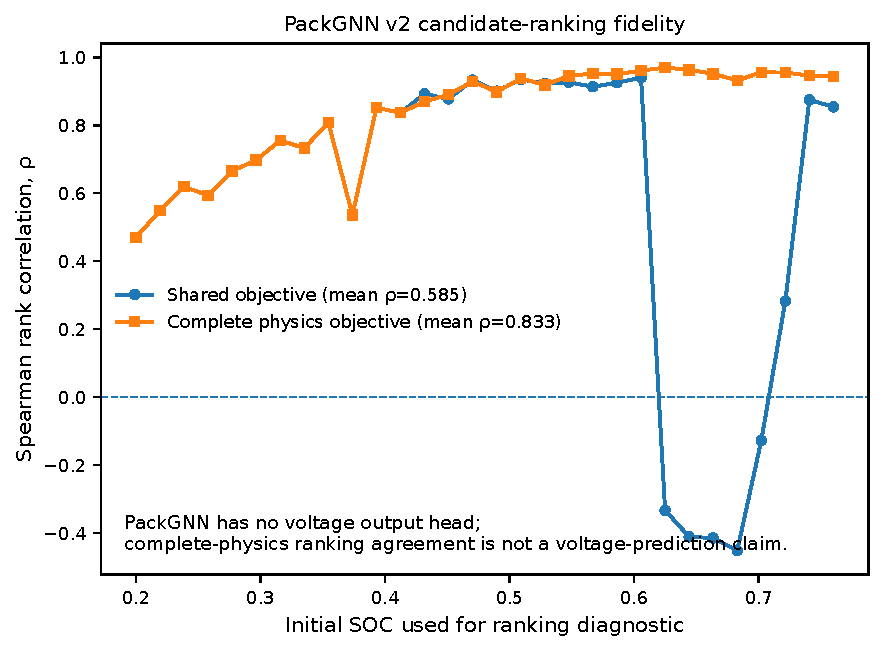
\includegraphics[width=\columnwidth]{figures/submission_v2/fig5_surrogate_ranking_fidelity.pdf}
\caption{Candidate-ranking fidelity of PackGNN v2 over 30 independent diagnostic states and 64 candidates per state. Spearman correlation is reported against the shared surrogate-compatible objective and the complete downstream physics objective. Ranking is generally informative but is not uniform across the full SOC range.}
\label{fig:ranking_fidelity}
\end{figure}

% SUPPLEMENTARY FIGURE S1
\begin{figure}[t]
\centering
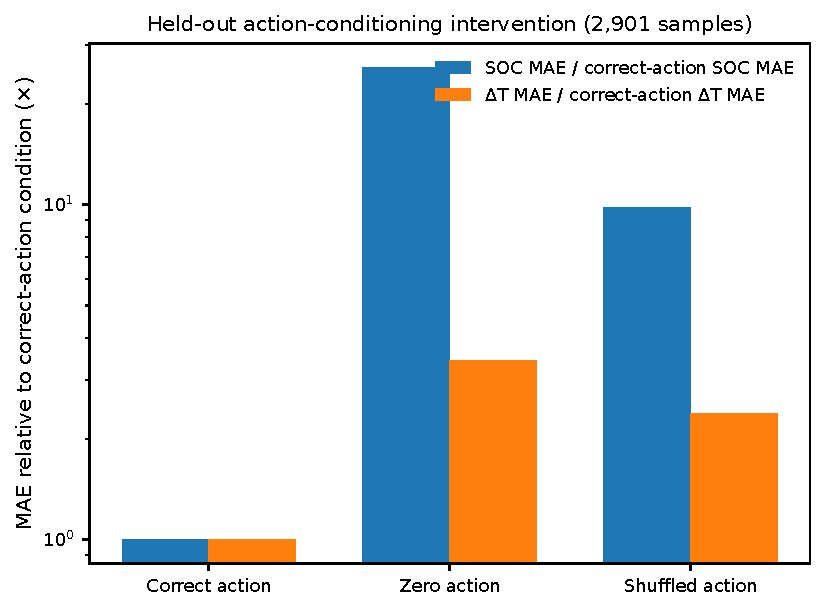
\includegraphics[width=\columnwidth]{figures/submission_v2/figS1_action_conditioning.pdf}
\caption{Held-out action-conditioning intervention. Zeroing or shuffling the candidate-action input substantially increases both SOC and temperature-change prediction error relative to the correct-action condition, supporting genuine action sensitivity of PackGNN v2.}
\label{fig:action_conditioning}
\end{figure}
